The Channel System(CS) that represents the C2 System ($CS_{C2}$) is composed by program graphs (PG) that represents the three roles identified as part of the system, i.e., C2 Approach Selector (C2A), Task Allocator (TA) and Executor (EX). The member or individuals can execute one or more roles simultaneously.

Our CS is parameterized, i.e., the program graphs instantiating is done according to the parameters passed. The parameters are the following:
\begin{itemize}
    \item T : set of tasks that defines the initial mission
    \item E : set of members $e_i$ that composes the team that is defined by the tuples $\langle FM, c_0\rangle$, where $FM$ is the feature model and $c_0$ is the initial valid configuration of the FM. 
    \item $\omega_0$ : the initial C2 approach ($C2_{ap}$) operated by the system
\end{itemize}

Based on this, we can define the CS as a parameterized function show by Equation \ref{function01}. Its graphical representation is shown by Figure \ref{cs01}.

\begin{equation}
\label{function01}
\begin{aligned}
CS_{C2}:&[e_1, e_2, ..., e_n]\ E,\ [t_1, t_2, ..., t_n]\ T,\ C2_{ap}\ \omega_0 \longrightarrow \\
&[C2A(E,T,\omega_0)\ |\ TA(\omega_0)\ |\ EX(e_1, \omega_0)\ |\ EX(e_2, \omega_0)\ |...|\ EX(e_n, \omega_0)]
\end{aligned}
\end{equation}

where each member $e_k$ of the list E of members, i.e., the team, is represented by the pair $e_k=\langle FM_k,c_{0_k} \rangle$ composed by the feature model and the initial configuration of the member, the $t_k$ is the k\textit{th} task of the set T, and $\omega_0$ is the initial C2 Approach ($C2_{ap}$) operated by the team E.

The total number of members, i.e., $n=|E|$, defines the quantity of Executor instances. Each PG that forms the CS receives attributes as argument in order to create the correct diagram and they are used to satisfy the initial guard condition $g_0$ of them.

\begin{equation}
\label{CS01}
    CS_{C2} = [C2A\ |\ TA\ |\ EX_1\ |\ EX_2\ |\ ...\ |\ EX_n]
\end{equation}

We can observe that C2A and TA roles appear only once even when instantiated. It occurs due to the crosscutting effect of these roles. Similar to features scattered by different components, these roles play as crosscutting concerns in the C2 System~\cite{Apel2013} and they can be executed by many individuals or members. On the other hand, the EX role is totally within a member and it is necessary to represent each instance as a member or process being executed, i.e., no feature scattering. Thus, C2A and TA roles can permeate the implementation of many members and it explains the representation in CS using only one role. 

\begin{figure}[h]
\centering
\label{cs01}
\scalebox{1}{


\tikzset{every picture/.style={line width=0.75pt}} %set default line width to 0.75pt        

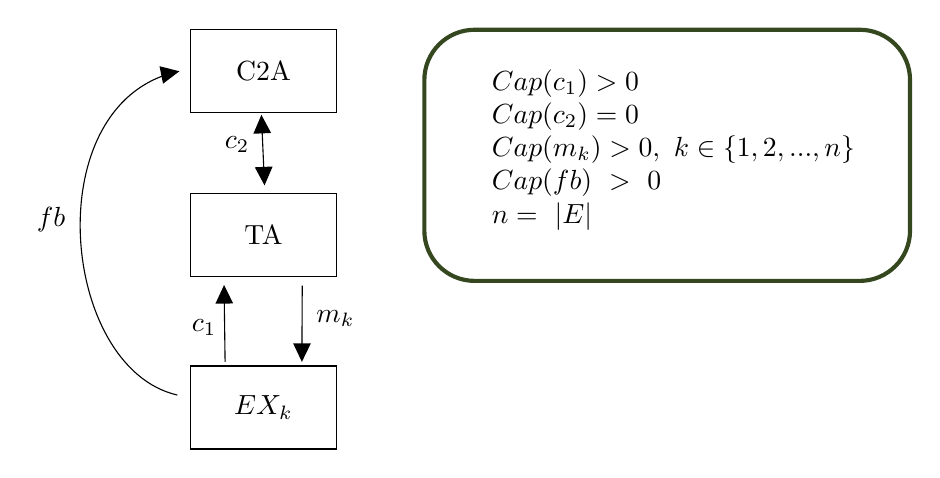
\begin{tikzpicture}[x=0.75pt,y=0.75pt,yscale=-1,xscale=1]
%uncomment if require: \path (0,229); %set diagram left start at 0, and has height of 229

%Shape: Rectangle [id:dp7793135649662085] 
\draw   (105,88) -- (175,88) -- (175,128) -- (105,128) -- cycle ;
%Shape: Rectangle [id:dp8388066725390221] 
\draw   (105,9) -- (175,9) -- (175,49) -- (105,49) -- cycle ;
%Shape: Rectangle [id:dp48691256180587716] 
\draw   (105,171) -- (175,171) -- (175,211) -- (105,211) -- cycle ;
%Straight Lines [id:da3337977868298102] 
\draw    (139.13,53) -- (140.37,81) ;
\draw [shift={(140.5,84)}, rotate = 267.47] [fill={rgb, 255:red, 0; green, 0; blue, 0 }  ][line width=0.08]  [draw opacity=0] (8.93,-4.29) -- (0,0) -- (8.93,4.29) -- cycle    ;
\draw [shift={(139,50)}, rotate = 87.47] [fill={rgb, 255:red, 0; green, 0; blue, 0 }  ][line width=0.08]  [draw opacity=0] (8.93,-4.29) -- (0,0) -- (8.93,4.29) -- cycle    ;
%Straight Lines [id:da7136052167478543] 
\draw    (158.67,132.33) -- (158.51,166) ;
\draw [shift={(158.5,169)}, rotate = 270.26] [fill={rgb, 255:red, 0; green, 0; blue, 0 }  ][line width=0.08]  [draw opacity=0] (8.93,-4.29) -- (0,0) -- (8.93,4.29) -- cycle    ;
%Straight Lines [id:da1199439366931846] 
\draw    (121.5,169) -- (121.04,135) ;
\draw [shift={(121,132)}, rotate = 449.23] [fill={rgb, 255:red, 0; green, 0; blue, 0 }  ][line width=0.08]  [draw opacity=0] (8.93,-4.29) -- (0,0) -- (8.93,4.29) -- cycle    ;
%Rounded Rect [id:dp3574279176331121] 
\draw  [color={rgb, 255:red, 53; green, 71; blue, 31 }  ,draw opacity=1 ][line width=1.5]  (217.5,33.2) .. controls (217.5,19.83) and (228.33,9) .. (241.7,9) -- (427.3,9) .. controls (440.67,9) and (451.5,19.83) .. (451.5,33.2) -- (451.5,105.8) .. controls (451.5,119.17) and (440.67,130) .. (427.3,130) -- (241.7,130) .. controls (228.33,130) and (217.5,119.17) .. (217.5,105.8) -- cycle ;
%Curve Lines [id:da7275055445236782] 
\draw    (98.5,185) .. controls (42.07,172.13) and (30.72,45.57) .. (97.45,29.45) ;
\draw [shift={(99.5,29)}, rotate = 528.53] [fill={rgb, 255:red, 0; green, 0; blue, 0 }  ][line width=0.08]  [draw opacity=0] (8.93,-4.29) -- (0,0) -- (8.93,4.29) -- cycle    ;

% Text Node
\draw (140,29) node   [align=left] {C2A};
% Text Node
\draw (140,108) node   [align=left] {TA};
% Text Node
\draw (140,191) node    {$EX_{k}$};
% Text Node
\draw (111.33,152.33) node    {$c_{1}$};
% Text Node
\draw (174.67,148) node    {$m_{k}$};
% Text Node
\draw (127.33,64.33) node    {$c_{2}$};
% Text Node
\draw (337.5,67) node    {$ \begin{array}{l}
Cap( c_{1})  >0\\
Cap( c_{2}) =0\\
Cap( m_{k})  >0,\ k\in \{1,2,...,n\}\\
Cap( fb) \  >\ 0\\
n=\ |E|\ 
\end{array}$};
% Text Node
\draw (37.67,100.67) node    {$fb$};


\end{tikzpicture}}
\caption{Channel System with its roles and channels represented}
\end{figure}

The formula \ref{CS01} represents the CS with $n$ instances of executors in a general view, that is represented by the following diagram.

\begin{figure}[h]
\centering
\label{cs02}
\scalebox{1}{

\tikzset{every picture/.style={line width=0.75pt}} %set default line width to 0.75pt        

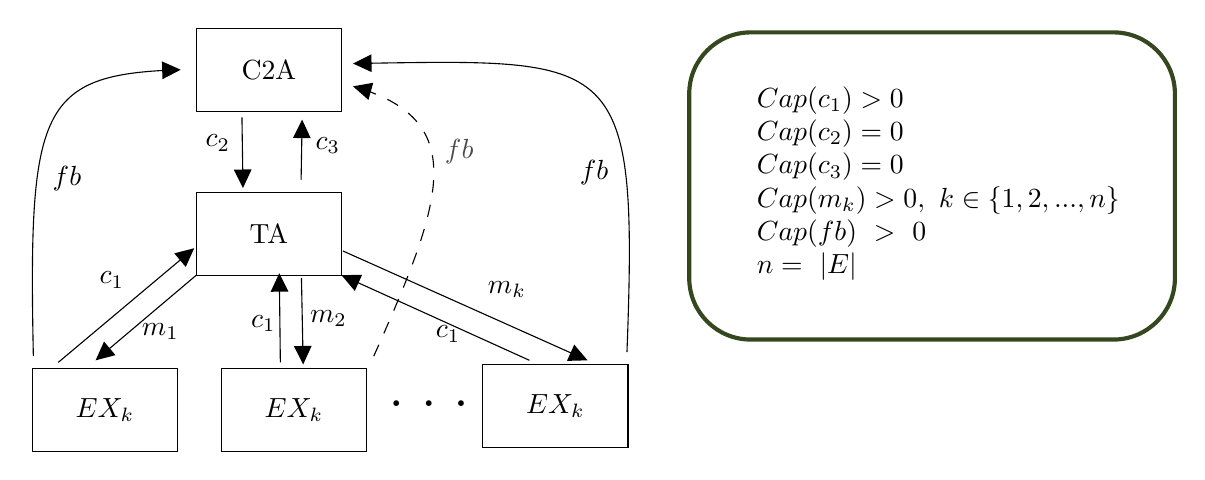
\begin{tikzpicture}[x=0.75pt,y=0.75pt,yscale=-1,xscale=1]
%uncomment if require: \path (0,229); %set diagram left start at 0, and has height of 229

%Shape: Rectangle [id:dp7793135649662085] 
\draw   (105,88) -- (175,88) -- (175,128) -- (105,128) -- cycle ;
%Shape: Rectangle [id:dp8388066725390221] 
\draw   (105,9) -- (175,9) -- (175,49) -- (105,49) -- cycle ;
%Shape: Rectangle [id:dp48691256180587716] 
\draw   (26,173) -- (96,173) -- (96,213) -- (26,213) -- cycle ;
%Straight Lines [id:da3337977868298102] 
\draw    (127,52) -- (127.46,83) ;
\draw [shift={(127.5,86)}, rotate = 269.15999999999997] [fill={rgb, 255:red, 0; green, 0; blue, 0 }  ][line width=0.08]  [draw opacity=0] (8.93,-4.29) -- (0,0) -- (8.93,4.29) -- cycle    ;
%Straight Lines [id:da7136052167478543] 
\draw    (155.67,129.33) -- (156.44,168) ;
\draw [shift={(156.5,171)}, rotate = 268.85] [fill={rgb, 255:red, 0; green, 0; blue, 0 }  ][line width=0.08]  [draw opacity=0] (8.93,-4.29) -- (0,0) -- (8.93,4.29) -- cycle    ;
%Straight Lines [id:da1199439366931846] 
\draw    (38.5,170) -- (101.7,116.93) ;
\draw [shift={(104,115)}, rotate = 499.98] [fill={rgb, 255:red, 0; green, 0; blue, 0 }  ][line width=0.08]  [draw opacity=0] (8.93,-4.29) -- (0,0) -- (8.93,4.29) -- cycle    ;
%Rounded Rect [id:dp3574279176331121] 
\draw  [color={rgb, 255:red, 53; green, 71; blue, 31 }  ,draw opacity=1 ][line width=1.5]  (342.5,40.6) .. controls (342.5,24.25) and (355.75,11) .. (372.1,11) -- (546.9,11) .. controls (563.25,11) and (576.5,24.25) .. (576.5,40.6) -- (576.5,129.4) .. controls (576.5,145.75) and (563.25,159) .. (546.9,159) -- (372.1,159) .. controls (355.75,159) and (342.5,145.75) .. (342.5,129.4) -- cycle ;
%Curve Lines [id:da7275055445236782] 
\draw    (26.5,167) .. controls (24.03,48.2) and (29.39,31.33) .. (95.48,29.06) ;
\draw [shift={(97.5,29)}, rotate = 538.3199999999999] [fill={rgb, 255:red, 0; green, 0; blue, 0 }  ][line width=0.08]  [draw opacity=0] (8.93,-4.29) -- (0,0) -- (8.93,4.29) -- cycle    ;
%Shape: Rectangle [id:dp8070909053866772] 
\draw   (243,171) -- (313,171) -- (313,211) -- (243,211) -- cycle ;
%Shape: Rectangle [id:dp18131918632628874] 
\draw   (117,173) -- (187,173) -- (187,213) -- (117,213) -- cycle ;
%Straight Lines [id:da4580469739796602] 
\draw    (145.5,170) -- (145.03,130) ;
\draw [shift={(145,127)}, rotate = 449.33] [fill={rgb, 255:red, 0; green, 0; blue, 0 }  ][line width=0.08]  [draw opacity=0] (8.93,-4.29) -- (0,0) -- (8.93,4.29) -- cycle    ;
%Straight Lines [id:da23459308482895536] 
\draw    (265.5,169) -- (177.73,129.24) ;
\draw [shift={(175,128)}, rotate = 384.37] [fill={rgb, 255:red, 0; green, 0; blue, 0 }  ][line width=0.08]  [draw opacity=0] (8.93,-4.29) -- (0,0) -- (8.93,4.29) -- cycle    ;
%Straight Lines [id:da9340034396500284] 
\draw    (175.67,116.33) -- (290.76,167.78) ;
\draw [shift={(293.5,169)}, rotate = 204.07999999999998] [fill={rgb, 255:red, 0; green, 0; blue, 0 }  ][line width=0.08]  [draw opacity=0] (8.93,-4.29) -- (0,0) -- (8.93,4.29) -- cycle    ;
%Straight Lines [id:da26523318096149495] 
\draw    (105,128) -- (58.79,167.06) ;
\draw [shift={(56.5,169)}, rotate = 319.78999999999996] [fill={rgb, 255:red, 0; green, 0; blue, 0 }  ][line width=0.08]  [draw opacity=0] (8.93,-4.29) -- (0,0) -- (8.93,4.29) -- cycle    ;
%Curve Lines [id:da641554832923748] 
\draw    (312.5,165) .. controls (317.97,20.72) and (308.59,23.96) .. (182.41,25.97) ;
\draw [shift={(180.5,26)}, rotate = 359.1] [fill={rgb, 255:red, 0; green, 0; blue, 0 }  ][line width=0.08]  [draw opacity=0] (8.93,-4.29) -- (0,0) -- (8.93,4.29) -- cycle    ;
%Curve Lines [id:da09438027167232854] 
\draw  [dash pattern={on 4.5pt off 4.5pt}]  (190.5,167) .. controls (223.5,93.12) and (237.09,54.18) .. (183.02,37.74) ;
\draw [shift={(180.5,37)}, rotate = 375.68] [fill={rgb, 255:red, 0; green, 0; blue, 0 }  ][line width=0.08]  [draw opacity=0] (8.93,-4.29) -- (0,0) -- (8.93,4.29) -- cycle    ;
%Straight Lines [id:da9905404427936819] 
\draw    (155.95,56) -- (155.5,82) ;
\draw [shift={(156,53)}, rotate = 90.99] [fill={rgb, 255:red, 0; green, 0; blue, 0 }  ][line width=0.08]  [draw opacity=0] (8.93,-4.29) -- (0,0) -- (8.93,4.29) -- cycle    ;

% Text Node
\draw (140,29) node   [align=left] {C2A};
% Text Node
\draw (140,108) node   [align=left] {TA};
% Text Node
\draw (61,193) node    {$EX_{k}$};
% Text Node
\draw (64.33,130.33) node    {$c_{1}$};
% Text Node
\draw (168.67,149) node    {$m_{2}$};
% Text Node
\draw (115.33,64.33) node    {$c_{2}$};
% Text Node
\draw (462.5,84) node    {$ \begin{array}{l}
Cap( c_{1})  >0\\
Cap( c_{2}) =0\\
Cap( c_{3}) =0\\
Cap( m_{k})  >0,\ k\in \{1,2,...,n\}\\
Cap( fb) \  >\ 0\\
n=\ |E|\ 
\end{array}$};
% Text Node
\draw (42.67,81.67) node    {$fb$};
% Text Node
\draw (278,191) node    {$EX_{k}$};
% Text Node
\draw (152,193) node    {$EX_{k}$};
% Text Node
\draw (217,190) node  [font=\Large] [align=left] {\textbf{. . .}};
% Text Node
\draw (254.67,135) node    {$m_{k}$};
% Text Node
\draw (87.67,155) node    {$m_{1}$};
% Text Node
\draw (137.33,151.33) node    {$c_{1}$};
% Text Node
\draw (226.33,156.33) node    {$c_{1}$};
% Text Node
\draw (296.67,78.67) node    {$fb$};
% Text Node
\draw (231.67,68.67) node  [color={rgb, 255:red, 74; green, 74; blue, 74 }  ,opacity=1 ]  {$fb$};
% Text Node
\draw (168.33,65.33) node    {$c_{3}$};


\end{tikzpicture}}
\caption{Channel System with PG instances}
\end{figure}

Based on this, we can find two different views. The first one is according to the roles, where they have the implementation spread among different individuals. It characterizes a crosscutting concern. However, we have another view under the member perspective. That view is defined by a tangled role in case of partial or total implementation and/or execution in different individuals or entities. 
The TS resulted from \ref{CS01} unfolded is a set of tuples in the form:

\begin{equation}
\label{CS02}
    TS(CS_{C2})=\langle l_{C2A}, l_{TA}, l_{EX_k}, \eta, \xi \rangle |_{k=1}^n
\end{equation}

where $l_p$ is the locate $l$ for the PG $p$, $\eta \in Eval(val)$ is the value of all variables in TS and $\xi$ is the state of all channels in the system, i.e., $lenght(\xi(c)) \leq cap(c), c \in \{c_1, c_2, m_1, ..., m_n, fb\}$.


When there are no context changes, the execution occurs normally and the steps are defined as:

\begin{enumerate}
    \item Select C2A
    \item Task allocation
    \item Member configuration
    \item Task execution
    \item Success report
\end{enumerate}

All other possible situations treated at this first stage is shown in Table \ref{table:scenarios}. The dynamic context includes possible changes in the self, mission or environment.

% \usepackage[normalem]{ulem}
% \usepackage{tablefootnote}
% \usepackage{colortbl}


\begin{table}[h!]
\centering
\fontsize{11}{11}\selectfont
\label{table:scenarios}
\begin{tabular}{|l|l|l|} 
\hline
\multicolumn{3}{|c|}{{\cellcolor[rgb]{0.753,0.753,0.753}}\textbf{Self} }\\ 
\hline
\multicolumn{3}{|c|}{\textbf{Sensor } }\\ 
\hline
\begin{tabular}[c]{@{}l@{}}1. Select C2A\\2. Task allocation\\3. Member configuration\\4. Task execution\\\textbf{\uline{5. Sensor issue}}\\\textbf{\uline{6. Member reconfiguration}}\\7. Task execution\\8. Success report \end{tabular}                                             & \begin{tabular}[c]{@{}l@{}}1. Select C2A\\2. Task allocation\\3. Member configuration\\4. Task execution\\\textbf{\uline{5. Sensor issue}}\\\textbf{\uline{6. Task reallocation}}\\\textbf{\uline{7. Member configuration\tablefootnote{Come configuration can be required in order to deal with the new tasks received after reallocation;}}}\\8. Task execution\\9. Success report \end{tabular} & \begin{tabular}[c]{@{}l@{}}1. Select C2A\\2. Task allocation\\3. Member configuration\\4. Task execution\\\textbf{\uline{5. Sensor issue}}\\\textbf{\uline{6. C2A selection\tablefootnote{In case of no solution with a reallocation, the problem is escalated to the C2 Approach selector;}}}\\\textbf{\uline{7. Task allocation}}\\\textbf{\uline{8. Member configuration}}\\9. Task execution\\10. Success report \end{tabular}             \\ 
\hline
\multicolumn{3}{|c|}{\textbf{Member} }\\ 
\hline
\multicolumn{2}{|l|}{\begin{tabular}[c]{@{}l@{}}1. Select C2A\\2. Task allocation\\3. Member configuration\\4. Task execution\\\textbf{\uline{5. Member issue}}\tablefootnote{In case of a member loosing and its tasks will be reallocated;}\\\textbf{\uline{6. Task reallocation}}\\\textbf{\uline{7. Member configuration}}\\8. Task execution\\9. Success report \end{tabular}}& \begin{tabular}[c]{@{}l@{}}1. Select C2A\\2. Task allocation\\3. Member configuration\\4. Task execution\\\textbf{\uline{5. Member issue}}\tablefootnote{the loss of any member will be staggered to a new C2 Approach selection;}\\\textbf{\uline{6. C2A selection}}\\\textbf{\uline{7. Task allocation}}\\\textbf{\uline{8. Member configuration}}\\9. Task execution\\10. Success report \end{tabular}  \\ 
\hline
\rowcolor[rgb]{0.753,0.753,0.753} \multicolumn{1}{|c|}{\textbf{Mission} }& \multicolumn{2}{c|}{ \textbf{Environment}}\\ 
\hline
\multicolumn{1}{|c|}{\textbf{Add/Remove Task}}& \multicolumn{1}{c|}{\textbf{Weather}}   \multicolumn{1}{c|}{\textbf{Hazard}}\\ 
\hline
\begin{tabular}[c]{@{}l@{}}1. Select C2A\\2. Task allocation\\3. Member configuration\\4. Task execution\\\textbf{\uline{5. Tasks added/removed}}\\\textbf{\uline{6. Task reallocation}}\\\textbf{\uline{7. Member configuration}}\\8. Task execution\\9. Success report \end{tabular} & \multicolumn{2}{l|}{Assumption: the same possibilities of Self changes}\\
\hline
\end{tabular}
\end{table}

The PG of each role are the following:

\begin{figure}[h!]
\centering
\label{PG001}
\scalebox{.8}{


\tikzset{every picture/.style={line width=0.75pt}} %set default line width to 0.75pt        

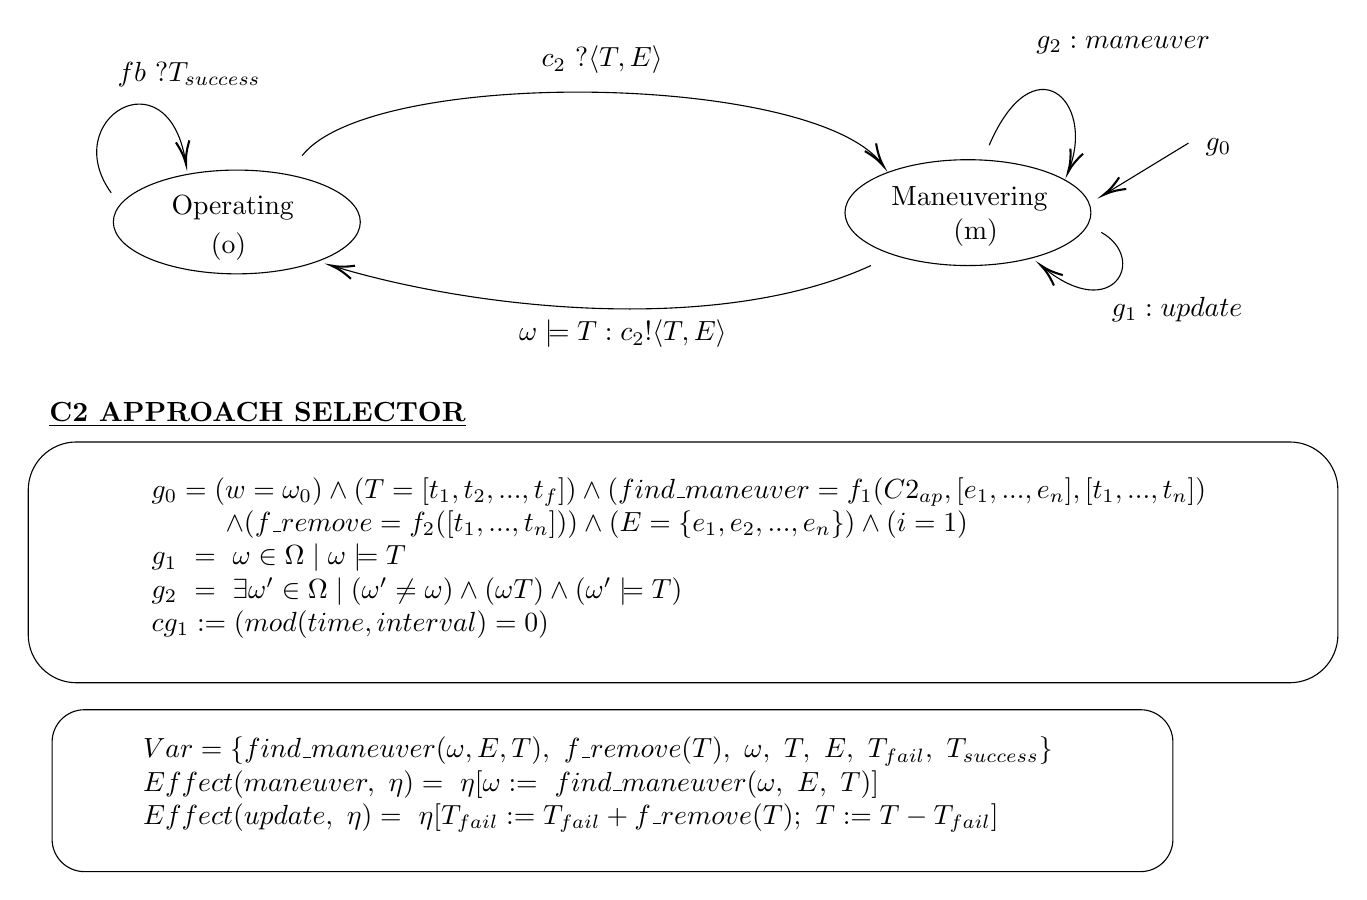
\begin{tikzpicture}[x=0.75pt,y=0.75pt,yscale=-1,xscale=1]
%uncomment if require: \path (0,420); %set diagram left start at 0, and has height of 420

%Curve Lines [id:da9480858267519683] 
\draw    (135.5,66) .. controls (169.16,23.43) and (380.22,25.94) .. (414.52,69.66) ;
\draw [shift={(415.5,71)}, rotate = 235.44] [color={rgb, 255:red, 0; green, 0; blue, 0 }  ][line width=0.75]    (10.93,-3.29) .. controls (6.95,-1.4) and (3.31,-0.3) .. (0,0) .. controls (3.31,0.3) and (6.95,1.4) .. (10.93,3.29)   ;
%Shape: Ellipse [id:dp6594609066072359] 
\draw   (44.5,98) .. controls (44.5,84.19) and (71.14,73) .. (104,73) .. controls (136.86,73) and (163.5,84.19) .. (163.5,98) .. controls (163.5,111.81) and (136.86,123) .. (104,123) .. controls (71.14,123) and (44.5,111.81) .. (44.5,98) -- cycle ;
%Shape: Ellipse [id:dp873836537729809] 
\draw   (397,93.5) .. controls (397,79.42) and (423.53,68) .. (456.25,68) .. controls (488.97,68) and (515.5,79.42) .. (515.5,93.5) .. controls (515.5,107.58) and (488.97,119) .. (456.25,119) .. controls (423.53,119) and (397,107.58) .. (397,93.5) -- cycle ;
%Curve Lines [id:da21020703050779688] 
\draw    (466.5,61) .. controls (487.68,11.75) and (517.59,39.15) .. (505.1,72.47) ;
\draw [shift={(504.5,74)}, rotate = 292.38] [color={rgb, 255:red, 0; green, 0; blue, 0 }  ][line width=0.75]    (10.93,-3.29) .. controls (6.95,-1.4) and (3.31,-0.3) .. (0,0) .. controls (3.31,0.3) and (6.95,1.4) .. (10.93,3.29)   ;
%Curve Lines [id:da14662580418826565] 
\draw    (520.5,103) .. controls (543.16,115.81) and (526.03,147.04) .. (493.02,120.26) ;
\draw [shift={(491.5,119)}, rotate = 400.46000000000004] [color={rgb, 255:red, 0; green, 0; blue, 0 }  ][line width=0.75]    (10.93,-3.29) .. controls (6.95,-1.4) and (3.31,-0.3) .. (0,0) .. controls (3.31,0.3) and (6.95,1.4) .. (10.93,3.29)   ;
%Straight Lines [id:da37650774099478246] 
\draw    (562.5,60) -- (523.21,83.96) ;
\draw [shift={(521.5,85)}, rotate = 328.63] [color={rgb, 255:red, 0; green, 0; blue, 0 }  ][line width=0.75]    (10.93,-3.29) .. controls (6.95,-1.4) and (3.31,-0.3) .. (0,0) .. controls (3.31,0.3) and (6.95,1.4) .. (10.93,3.29)   ;
%Rounded Rect [id:dp20897962983691354] 
\draw   (3.5,227.2) .. controls (3.5,214.39) and (13.89,204) .. (26.7,204) -- (611.3,204) .. controls (624.11,204) and (634.5,214.39) .. (634.5,227.2) -- (634.5,296.8) .. controls (634.5,309.61) and (624.11,320) .. (611.3,320) -- (26.7,320) .. controls (13.89,320) and (3.5,309.61) .. (3.5,296.8) -- cycle ;
%Rounded Rect [id:dp6489541210438411] 
\draw   (15,348.6) .. controls (15,339.98) and (21.98,333) .. (30.6,333) -- (539.4,333) .. controls (548.02,333) and (555,339.98) .. (555,348.6) -- (555,395.4) .. controls (555,404.02) and (548.02,411) .. (539.4,411) -- (30.6,411) .. controls (21.98,411) and (15,404.02) .. (15,395.4) -- cycle ;
%Curve Lines [id:da07722007259294938] 
\draw    (43.5,84) .. controls (17.76,48.36) and (70.43,16.64) .. (79.25,68.41) ;
\draw [shift={(79.5,70)}, rotate = 261.57] [color={rgb, 255:red, 0; green, 0; blue, 0 }  ][line width=0.75]    (10.93,-3.29) .. controls (6.95,-1.4) and (3.31,-0.3) .. (0,0) .. controls (3.31,0.3) and (6.95,1.4) .. (10.93,3.29)   ;
%Curve Lines [id:da13961356622291943] 
\draw    (409.5,119) .. controls (335.87,152.83) and (218.68,140.13) .. (150.52,119.31) ;
\draw [shift={(149.5,119)}, rotate = 377.15999999999997] [color={rgb, 255:red, 0; green, 0; blue, 0 }  ][line width=0.75]    (10.93,-3.29) .. controls (6.95,-1.4) and (3.31,-0.3) .. (0,0) .. controls (3.31,0.3) and (6.95,1.4) .. (10.93,3.29)   ;

% Text Node
\draw (102,91) node   [align=left] {Operating};
% Text Node
\draw (457,87) node   [align=left] {Maneuvering};
% Text Node
\draw (280,20) node    {$c_{2} \ ?\langle T,E\rangle $};
% Text Node
\draw (577,62) node    {$g_{0}$};
% Text Node
\draw (557,140) node    {$g_{1} :update$};
% Text Node
\draw (531,13) node    {$g_{2} :maneuver$};
% Text Node
\draw (317,260) node    {$ \begin{array}{l}
g_{0} =( w=\omega _{0}) \land ( T=[ t_{1} ,t_{2} ,...,t_{f}]) \land ( find\_maneuver=f_{1}( C2_{ap} ,[ e_{1} ,...,e_{n}] ,[ t_{1} ,...,t_{n}])\\
\ \ \ \ \ \ \ \ \land ( f\_remove=f_{2}([ t_{1} ,...,t_{n}])) \land ( E=\{e_{1} ,e_{2} ,...,e_{n}\}) \land ( i=1)\\
g_{1} \ =\ \nexists \omega \in \Omega \mid \omega \models T\\
g_{2} \ =\ \exists \omega '\in \Omega \mid ( \omega '\neq \omega ) \land ( \omega \nvDash T) \land ( \omega '\models T)\\
cg_{1} :=( mod( time,interval) =0)
\end{array}$};
% Text Node
\draw (460,103) node   [align=left] {(m)};
% Text Node
\draw (100,110) node   [align=left] {(o)};
% Text Node
\draw (278,369) node    {$ \begin{array}{l}
Var=\{find\_maneuver( \omega ,E,T) ,\ f\_remove( T) ,\ \omega ,\ T,\ E,\ T_{fail} ,\ T_{success}\}\\
Effect( maneuver,\ \eta ) =\ \eta [ \omega :=\ find\_maneuver( \omega ,\ E,\ T)]\\
Effect( update,\ \eta ) =\ \eta [ T_{fail} :=T_{fail} +f\_remove( T) ;\ T:=T-T_{fail}]
\end{array}$};
% Text Node
\draw (81,27) node    {$fb\ ?T_{success}$};
% Text Node
\draw (114,191) node   [align=left] {\textbf{\underline{C2 APPROACH SELECTOR}}};
% Text Node
\draw (290,152) node    {$\omega \models T:c_{2} !\langle T,E\rangle $};


\end{tikzpicture}}
\caption{C2 Approach Selector PG}
\end{figure}


\begin{figure}[h!]
\centering
\label{PG002}
\scalebox{.8}{\input{tiks/ta}}
\caption{Task Allocator PG}
\end{figure}


\begin{figure}[h!]
\centering
\label{PG003}
\scalebox{.8}{

\tikzset{every picture/.style={line width=0.75pt}} %set default line width to 0.75pt        

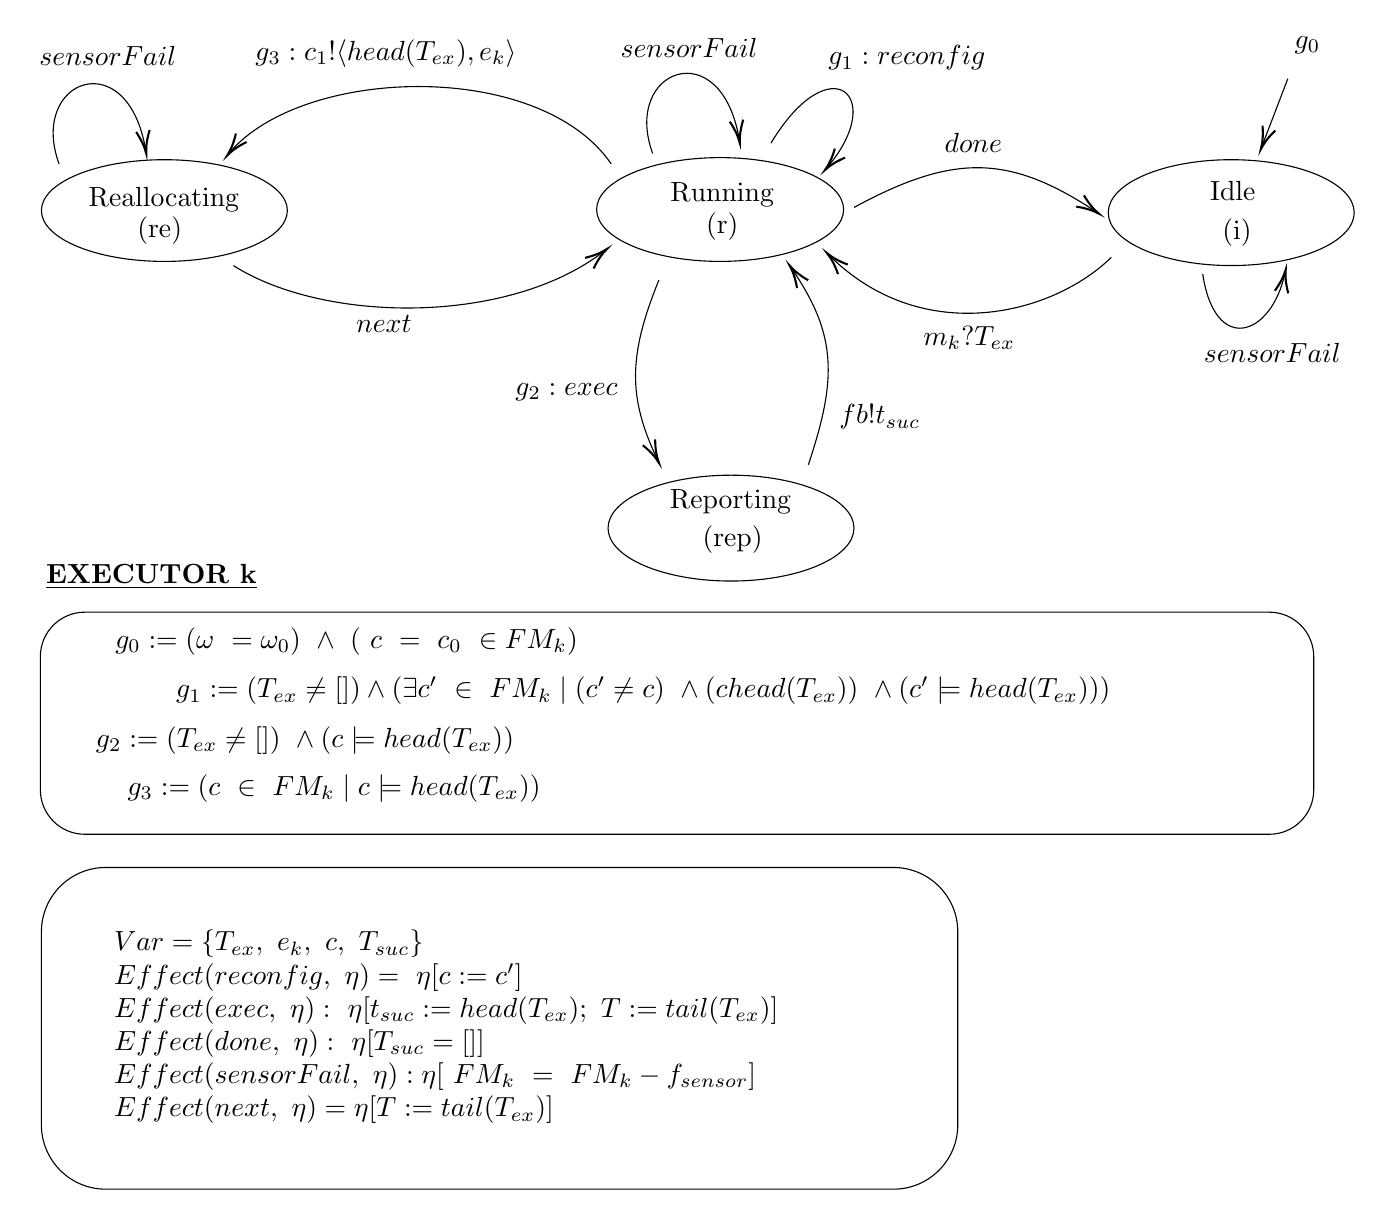
\begin{tikzpicture}[x=0.75pt,y=0.75pt,yscale=-1,xscale=1]
%uncomment if require: \path (0,582); %set diagram left start at 0, and has height of 582

%Curve Lines [id:da9480858267519683] 
\draw    (385.5,222) .. controls (399.29,180.63) and (399.5,159.63) .. (377.52,127.48) ;
\draw [shift={(376.5,126)}, rotate = 415.12] [color={rgb, 255:red, 0; green, 0; blue, 0 }  ][line width=0.75]    (10.93,-3.29) .. controls (6.95,-1.4) and (3.31,-0.3) .. (0,0) .. controls (3.31,0.3) and (6.95,1.4) .. (10.93,3.29)   ;
%Shape: Ellipse [id:dp6594609066072359] 
\draw   (283.5,99) .. controls (283.5,85.19) and (310.14,74) .. (343,74) .. controls (375.86,74) and (402.5,85.19) .. (402.5,99) .. controls (402.5,112.81) and (375.86,124) .. (343,124) .. controls (310.14,124) and (283.5,112.81) .. (283.5,99) -- cycle ;
%Shape: Ellipse [id:dp873836537729809] 
\draw   (530,100.5) .. controls (530,86.42) and (556.53,75) .. (589.25,75) .. controls (621.97,75) and (648.5,86.42) .. (648.5,100.5) .. controls (648.5,114.58) and (621.97,126) .. (589.25,126) .. controls (556.53,126) and (530,114.58) .. (530,100.5) -- cycle ;
%Curve Lines [id:da21020703050779688] 
\draw    (367.5,67) .. controls (396.21,19.48) and (423.94,44.49) .. (394.41,78.95) ;
\draw [shift={(393.5,80)}, rotate = 311.53] [color={rgb, 255:red, 0; green, 0; blue, 0 }  ][line width=0.75]    (10.93,-3.29) .. controls (6.95,-1.4) and (3.31,-0.3) .. (0,0) .. controls (3.31,0.3) and (6.95,1.4) .. (10.93,3.29)   ;
%Straight Lines [id:da37650774099478246] 
\draw    (616.5,36) -- (604.21,68.13) ;
\draw [shift={(603.5,70)}, rotate = 290.92] [color={rgb, 255:red, 0; green, 0; blue, 0 }  ][line width=0.75]    (10.93,-3.29) .. controls (6.95,-1.4) and (3.31,-0.3) .. (0,0) .. controls (3.31,0.3) and (6.95,1.4) .. (10.93,3.29)   ;
%Shape: Ellipse [id:dp02234558999259495] 
\draw   (16,99.5) .. controls (16,85.97) and (42.53,75) .. (75.25,75) .. controls (107.97,75) and (134.5,85.97) .. (134.5,99.5) .. controls (134.5,113.03) and (107.97,124) .. (75.25,124) .. controls (42.53,124) and (16,113.03) .. (16,99.5) -- cycle ;
%Curve Lines [id:da2517277021570281] 
\draw    (290.5,77) .. controls (255.85,26.51) and (141.81,29.93) .. (106.54,71.72) ;
\draw [shift={(105.5,73)}, rotate = 308.33000000000004] [color={rgb, 255:red, 0; green, 0; blue, 0 }  ][line width=0.75]    (10.93,-3.29) .. controls (6.95,-1.4) and (3.31,-0.3) .. (0,0) .. controls (3.31,0.3) and (6.95,1.4) .. (10.93,3.29)   ;
%Curve Lines [id:da851947022127026] 
\draw    (108.5,126) .. controls (152.06,153.72) and (240.7,154.98) .. (287.11,119.1) ;
\draw [shift={(288.5,118)}, rotate = 501.19] [color={rgb, 255:red, 0; green, 0; blue, 0 }  ][line width=0.75]    (10.93,-3.29) .. controls (6.95,-1.4) and (3.31,-0.3) .. (0,0) .. controls (3.31,0.3) and (6.95,1.4) .. (10.93,3.29)   ;
%Curve Lines [id:da05773774536505705] 
\draw    (531.5,122) .. controls (503.29,149.72) and (440.77,165.68) .. (395.86,121.36) ;
\draw [shift={(394.5,120)}, rotate = 405.63] [color={rgb, 255:red, 0; green, 0; blue, 0 }  ][line width=0.75]    (10.93,-3.29) .. controls (6.95,-1.4) and (3.31,-0.3) .. (0,0) .. controls (3.31,0.3) and (6.95,1.4) .. (10.93,3.29)   ;
%Rounded Rect [id:dp5913972444482631] 
\draw   (15.5,314.4) .. controls (15.5,302.58) and (25.08,293) .. (36.9,293) -- (607.6,293) .. controls (619.42,293) and (629,302.58) .. (629,314.4) -- (629,378.6) .. controls (629,390.42) and (619.42,400) .. (607.6,400) -- (36.9,400) .. controls (25.08,400) and (15.5,390.42) .. (15.5,378.6) -- cycle ;
%Rounded Rect [id:dp9206164489184118] 
\draw   (16,447) .. controls (16,429.88) and (29.88,416) .. (47,416) -- (426.5,416) .. controls (443.62,416) and (457.5,429.88) .. (457.5,447) -- (457.5,540) .. controls (457.5,557.12) and (443.62,571) .. (426.5,571) -- (47,571) .. controls (29.88,571) and (16,557.12) .. (16,540) -- cycle ;
%Curve Lines [id:da46585089178877326] 
\draw    (24.5,77) .. controls (9.65,36.41) and (57.53,18.36) .. (66.25,70.4) ;
\draw [shift={(66.5,72)}, rotate = 261.57] [color={rgb, 255:red, 0; green, 0; blue, 0 }  ][line width=0.75]    (10.93,-3.29) .. controls (6.95,-1.4) and (3.31,-0.3) .. (0,0) .. controls (3.31,0.3) and (6.95,1.4) .. (10.93,3.29)   ;
%Curve Lines [id:da24525569786800605] 
\draw    (575.5,130) .. controls (581.38,169.2) and (608.39,160.38) .. (615.11,129.89) ;
\draw [shift={(615.5,128)}, rotate = 460.62] [color={rgb, 255:red, 0; green, 0; blue, 0 }  ][line width=0.75]    (10.93,-3.29) .. controls (6.95,-1.4) and (3.31,-0.3) .. (0,0) .. controls (3.31,0.3) and (6.95,1.4) .. (10.93,3.29)   ;
%Curve Lines [id:da5617910694928671] 
\draw    (310.5,72) .. controls (295.65,31.41) and (343.53,13.36) .. (352.25,65.4) ;
\draw [shift={(352.5,67)}, rotate = 261.57] [color={rgb, 255:red, 0; green, 0; blue, 0 }  ][line width=0.75]    (10.93,-3.29) .. controls (6.95,-1.4) and (3.31,-0.3) .. (0,0) .. controls (3.31,0.3) and (6.95,1.4) .. (10.93,3.29)   ;
%Shape: Ellipse [id:dp893416141673501] 
\draw   (289,252.5) .. controls (289,238.42) and (315.53,227) .. (348.25,227) .. controls (380.97,227) and (407.5,238.42) .. (407.5,252.5) .. controls (407.5,266.58) and (380.97,278) .. (348.25,278) .. controls (315.53,278) and (289,266.58) .. (289,252.5) -- cycle ;
%Curve Lines [id:da2982425830385871] 
\draw    (313.5,133) .. controls (298.72,169.45) and (298.5,189.4) .. (312.84,219.61) ;
\draw [shift={(313.5,221)}, rotate = 244.18] [color={rgb, 255:red, 0; green, 0; blue, 0 }  ][line width=0.75]    (10.93,-3.29) .. controls (6.95,-1.4) and (3.31,-0.3) .. (0,0) .. controls (3.31,0.3) and (6.95,1.4) .. (10.93,3.29)   ;
%Curve Lines [id:da08998093824564413] 
\draw    (407.5,98) .. controls (455.02,72.26) and (481.96,72) .. (524.21,100.14) ;
\draw [shift={(525.5,101)}, rotate = 214] [color={rgb, 255:red, 0; green, 0; blue, 0 }  ][line width=0.75]    (10.93,-3.29) .. controls (6.95,-1.4) and (3.31,-0.3) .. (0,0) .. controls (3.31,0.3) and (6.95,1.4) .. (10.93,3.29)   ;

% Text Node
\draw (344,92) node   [align=left] {Running};
% Text Node
\draw (590,90) node   [align=left] {Idle};
% Text Node
\draw (420,199) node    {$fb!t_{suc}$};
% Text Node
\draw (182,24) node    {$g_{3} :c_{1} !\langle head( T_{ex}) ,e_{k} \rangle $};
% Text Node
\draw (463,161) node    {$m_{k} ?T_{ex}$};
% Text Node
\draw (75,94) node   [align=left] {Reallocating};
% Text Node
\draw (181,154) node    {$next$};
% Text Node
\draw (306,331) node    {$g_{1} :=( T_{ex} \neq []) \land ( \exists c'\ \in \ \llbracket FM_{k} \rrbracket \mid ( c'\neq c) \ \land ( c\nvDash head( T_{ex})) \ \land ( c'\models head( T_{ex})))$};
% Text Node
\draw (433,26) node    {$g_{1} :reconfig$};
% Text Node
\draw (269,187) node    {$g_{2} :exec$};
% Text Node
\draw (143,355) node    {$g_{2} :=( T_{ex} \neq []) \ \land ( c\models head( T_{ex}))$};
% Text Node
\draw (152,461) node    {$ \begin{array}{l}
\end{array}$};
% Text Node
\draw (211,493) node    {$ \begin{array}{l}
Var=\{T_{ex} ,\ e_{k} ,\ c,\ T_{suc}\}\\
Effect( reconfig,\ \eta ) =\ \eta [ c:=c']\\
Effect( exec,\ \eta ) :\ \eta [ t_{suc} :=head( T_{ex}) ;\ T:=tail( T_{ex})]\\
Effect( done,\ \eta ) :\ \eta [ T_{suc} =[]]\\
Effect( sensorFail,\ \eta ) :\eta [ \ FM_{k} \ =\ FM_{k} -f_{sensor}]\\
Effect( next,\ \eta ) =\eta [ T:=tail( T_{ex})]
\end{array}$};
% Text Node
\draw (73,109) node   [align=left] {(re)};
% Text Node
\draw (344,107) node   [align=left] {(r)};
% Text Node
\draw (592,110) node   [align=left] {(i)};
% Text Node
\draw (626,20) node    {$g_{0}$};
% Text Node
\draw (157,378) node    {$g_{3} :=( \nexists c\ \in \ \llbracket FM_{k} \rrbracket \mid c\models head( T_{ex}))$};
% Text Node
\draw (163,307) node    {$g_{0} :=( \omega \ =\omega _{0}) \ \land \ ( \ c\ =\ c_{0} \ \in \llbracket FM_{k} \rrbracket )$};
% Text Node
\draw (48,25) node    {$sensorFail$};
% Text Node
\draw (609,168) node    {$sensorFail$};
% Text Node
\draw (465,67) node    {$done$};
% Text Node
\draw (328,21) node    {$sensorFail$};
% Text Node
\draw (348,240) node   [align=left] {Reporting};
% Text Node
\draw (349,258) node   [align=left] {(rep)};
% Text Node
\draw (69,276) node   [align=left] {\textbf{\underline{EXECUTOR k}}};


\end{tikzpicture}}
\caption{Executor PG}
\end{figure}

According to possible situations considered and listed in Table \ref{table:scenarios}, we can unfold the PGs above and create the related TS.

\begin{figure}[h!]
\centering
\label{TS01}
\scalebox{.8}{


\tikzset{every picture/.style={line width=0.75pt}} %set default line width to 0.75pt        

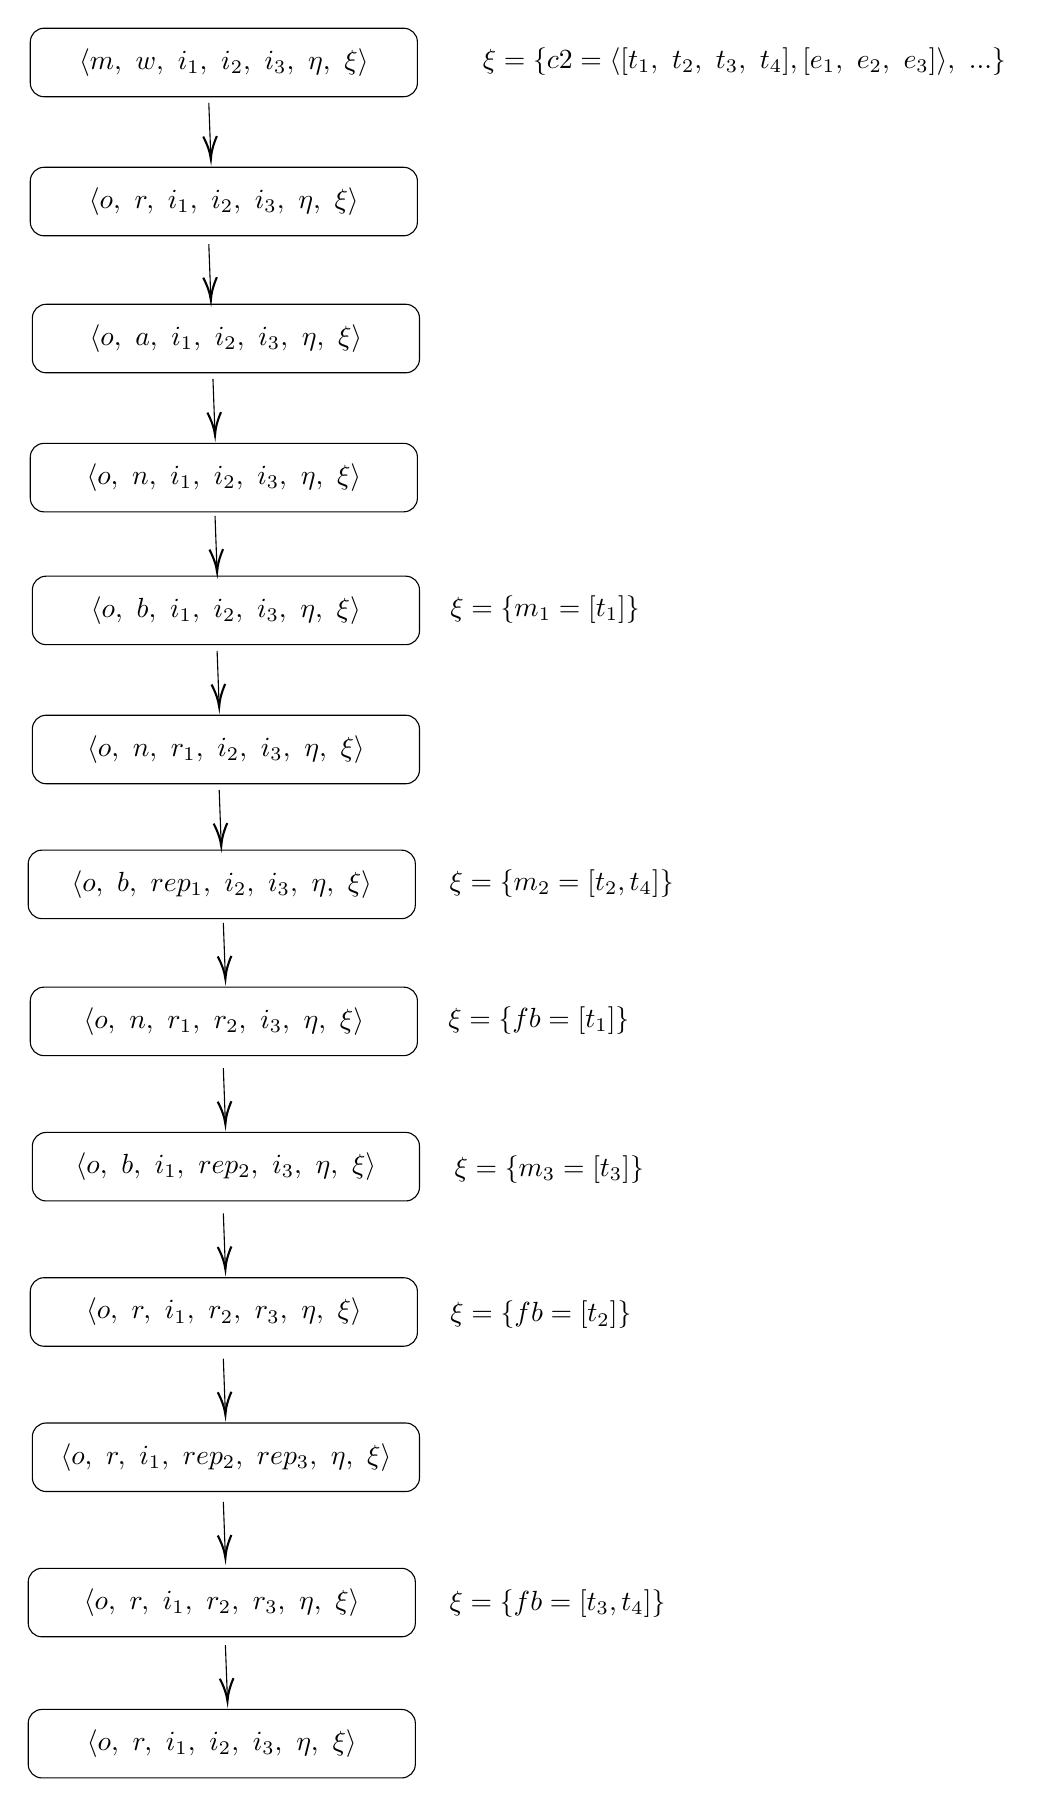
\begin{tikzpicture}[x=0.75pt,y=0.75pt,yscale=-1,xscale=1]
%uncomment if require: \path (0,865); %set diagram left start at 0, and has height of 865

%Rounded Rect [id:dp9048297129007524] 
\draw   (19,13.6) .. controls (19,9.95) and (21.95,7) .. (25.6,7) -- (198.9,7) .. controls (202.55,7) and (205.5,9.95) .. (205.5,13.6) -- (205.5,33.4) .. controls (205.5,37.05) and (202.55,40) .. (198.9,40) -- (25.6,40) .. controls (21.95,40) and (19,37.05) .. (19,33.4) -- cycle ;
%Rounded Rect [id:dp8152798292363221] 
\draw   (19,80.6) .. controls (19,76.95) and (21.95,74) .. (25.6,74) -- (198.9,74) .. controls (202.55,74) and (205.5,76.95) .. (205.5,80.6) -- (205.5,100.4) .. controls (205.5,104.05) and (202.55,107) .. (198.9,107) -- (25.6,107) .. controls (21.95,107) and (19,104.05) .. (19,100.4) -- cycle ;
%Rounded Rect [id:dp2611238064001401] 
\draw   (20,146.6) .. controls (20,142.95) and (22.95,140) .. (26.6,140) -- (199.9,140) .. controls (203.55,140) and (206.5,142.95) .. (206.5,146.6) -- (206.5,166.4) .. controls (206.5,170.05) and (203.55,173) .. (199.9,173) -- (26.6,173) .. controls (22.95,173) and (20,170.05) .. (20,166.4) -- cycle ;
%Rounded Rect [id:dp5474323622335151] 
\draw   (19,213.6) .. controls (19,209.95) and (21.95,207) .. (25.6,207) -- (198.9,207) .. controls (202.55,207) and (205.5,209.95) .. (205.5,213.6) -- (205.5,233.4) .. controls (205.5,237.05) and (202.55,240) .. (198.9,240) -- (25.6,240) .. controls (21.95,240) and (19,237.05) .. (19,233.4) -- cycle ;
%Rounded Rect [id:dp617967347556163] 
\draw   (20,277.6) .. controls (20,273.95) and (22.95,271) .. (26.6,271) -- (199.9,271) .. controls (203.55,271) and (206.5,273.95) .. (206.5,277.6) -- (206.5,297.4) .. controls (206.5,301.05) and (203.55,304) .. (199.9,304) -- (26.6,304) .. controls (22.95,304) and (20,301.05) .. (20,297.4) -- cycle ;
%Rounded Rect [id:dp6526355611328125] 
\draw   (20,344.6) .. controls (20,340.95) and (22.95,338) .. (26.6,338) -- (199.9,338) .. controls (203.55,338) and (206.5,340.95) .. (206.5,344.6) -- (206.5,364.4) .. controls (206.5,368.05) and (203.55,371) .. (199.9,371) -- (26.6,371) .. controls (22.95,371) and (20,368.05) .. (20,364.4) -- cycle ;
%Rounded Rect [id:dp6698610095556133] 
\draw   (18,409.6) .. controls (18,405.95) and (20.95,403) .. (24.6,403) -- (197.9,403) .. controls (201.55,403) and (204.5,405.95) .. (204.5,409.6) -- (204.5,429.4) .. controls (204.5,433.05) and (201.55,436) .. (197.9,436) -- (24.6,436) .. controls (20.95,436) and (18,433.05) .. (18,429.4) -- cycle ;
%Rounded Rect [id:dp9742586895494759] 
\draw   (19,475.6) .. controls (19,471.95) and (21.95,469) .. (25.6,469) -- (198.9,469) .. controls (202.55,469) and (205.5,471.95) .. (205.5,475.6) -- (205.5,495.4) .. controls (205.5,499.05) and (202.55,502) .. (198.9,502) -- (25.6,502) .. controls (21.95,502) and (19,499.05) .. (19,495.4) -- cycle ;
%Rounded Rect [id:dp34832491140564725] 
\draw   (20,545.6) .. controls (20,541.95) and (22.95,539) .. (26.6,539) -- (199.9,539) .. controls (203.55,539) and (206.5,541.95) .. (206.5,545.6) -- (206.5,565.4) .. controls (206.5,569.05) and (203.55,572) .. (199.9,572) -- (26.6,572) .. controls (22.95,572) and (20,569.05) .. (20,565.4) -- cycle ;
%Rounded Rect [id:dp07632153248409779] 
\draw   (19,615.6) .. controls (19,611.95) and (21.95,609) .. (25.6,609) -- (198.9,609) .. controls (202.55,609) and (205.5,611.95) .. (205.5,615.6) -- (205.5,635.4) .. controls (205.5,639.05) and (202.55,642) .. (198.9,642) -- (25.6,642) .. controls (21.95,642) and (19,639.05) .. (19,635.4) -- cycle ;
%Rounded Rect [id:dp38638906596830014] 
\draw   (20,685.6) .. controls (20,681.95) and (22.95,679) .. (26.6,679) -- (199.9,679) .. controls (203.55,679) and (206.5,681.95) .. (206.5,685.6) -- (206.5,705.4) .. controls (206.5,709.05) and (203.55,712) .. (199.9,712) -- (26.6,712) .. controls (22.95,712) and (20,709.05) .. (20,705.4) -- cycle ;
%Rounded Rect [id:dp2961818663412775] 
\draw   (18,755.6) .. controls (18,751.95) and (20.95,749) .. (24.6,749) -- (197.9,749) .. controls (201.55,749) and (204.5,751.95) .. (204.5,755.6) -- (204.5,775.4) .. controls (204.5,779.05) and (201.55,782) .. (197.9,782) -- (24.6,782) .. controls (20.95,782) and (18,779.05) .. (18,775.4) -- cycle ;
%Rounded Rect [id:dp1419509373702863] 
\draw   (18,823.6) .. controls (18,819.95) and (20.95,817) .. (24.6,817) -- (197.9,817) .. controls (201.55,817) and (204.5,819.95) .. (204.5,823.6) -- (204.5,843.4) .. controls (204.5,847.05) and (201.55,850) .. (197.9,850) -- (24.6,850) .. controls (20.95,850) and (18,847.05) .. (18,843.4) -- cycle ;
%Straight Lines [id:da25623652531692265] 
\draw    (105,43) -- (105.93,68) ;
\draw [shift={(106,70)}, rotate = 267.88] [color={rgb, 255:red, 0; green, 0; blue, 0 }  ][line width=0.75]    (10.93,-3.29) .. controls (6.95,-1.4) and (3.31,-0.3) .. (0,0) .. controls (3.31,0.3) and (6.95,1.4) .. (10.93,3.29)   ;
%Straight Lines [id:da9454848916406987] 
\draw    (105,111) -- (105.93,136) ;
\draw [shift={(106,138)}, rotate = 267.88] [color={rgb, 255:red, 0; green, 0; blue, 0 }  ][line width=0.75]    (10.93,-3.29) .. controls (6.95,-1.4) and (3.31,-0.3) .. (0,0) .. controls (3.31,0.3) and (6.95,1.4) .. (10.93,3.29)   ;
%Straight Lines [id:da9308850791504091] 
\draw    (107,176) -- (107.93,201) ;
\draw [shift={(108,203)}, rotate = 267.88] [color={rgb, 255:red, 0; green, 0; blue, 0 }  ][line width=0.75]    (10.93,-3.29) .. controls (6.95,-1.4) and (3.31,-0.3) .. (0,0) .. controls (3.31,0.3) and (6.95,1.4) .. (10.93,3.29)   ;
%Straight Lines [id:da6987828125639035] 
\draw    (108,242) -- (108.93,267) ;
\draw [shift={(109,269)}, rotate = 267.88] [color={rgb, 255:red, 0; green, 0; blue, 0 }  ][line width=0.75]    (10.93,-3.29) .. controls (6.95,-1.4) and (3.31,-0.3) .. (0,0) .. controls (3.31,0.3) and (6.95,1.4) .. (10.93,3.29)   ;
%Straight Lines [id:da38465000460546606] 
\draw    (109,307) -- (109.93,332) ;
\draw [shift={(110,334)}, rotate = 267.88] [color={rgb, 255:red, 0; green, 0; blue, 0 }  ][line width=0.75]    (10.93,-3.29) .. controls (6.95,-1.4) and (3.31,-0.3) .. (0,0) .. controls (3.31,0.3) and (6.95,1.4) .. (10.93,3.29)   ;
%Straight Lines [id:da7402304756808019] 
\draw    (110,374) -- (110.93,399) ;
\draw [shift={(111,401)}, rotate = 267.88] [color={rgb, 255:red, 0; green, 0; blue, 0 }  ][line width=0.75]    (10.93,-3.29) .. controls (6.95,-1.4) and (3.31,-0.3) .. (0,0) .. controls (3.31,0.3) and (6.95,1.4) .. (10.93,3.29)   ;
%Straight Lines [id:da32843301316145035] 
\draw    (112,438) -- (112.93,463) ;
\draw [shift={(113,465)}, rotate = 267.88] [color={rgb, 255:red, 0; green, 0; blue, 0 }  ][line width=0.75]    (10.93,-3.29) .. controls (6.95,-1.4) and (3.31,-0.3) .. (0,0) .. controls (3.31,0.3) and (6.95,1.4) .. (10.93,3.29)   ;
%Straight Lines [id:da33931279270538006] 
\draw    (112,508) -- (112.93,533) ;
\draw [shift={(113,535)}, rotate = 267.88] [color={rgb, 255:red, 0; green, 0; blue, 0 }  ][line width=0.75]    (10.93,-3.29) .. controls (6.95,-1.4) and (3.31,-0.3) .. (0,0) .. controls (3.31,0.3) and (6.95,1.4) .. (10.93,3.29)   ;
%Straight Lines [id:da4793309632596934] 
\draw    (112,578) -- (112.93,603) ;
\draw [shift={(113,605)}, rotate = 267.88] [color={rgb, 255:red, 0; green, 0; blue, 0 }  ][line width=0.75]    (10.93,-3.29) .. controls (6.95,-1.4) and (3.31,-0.3) .. (0,0) .. controls (3.31,0.3) and (6.95,1.4) .. (10.93,3.29)   ;
%Straight Lines [id:da7517013161282193] 
\draw    (112,648) -- (112.93,673) ;
\draw [shift={(113,675)}, rotate = 267.88] [color={rgb, 255:red, 0; green, 0; blue, 0 }  ][line width=0.75]    (10.93,-3.29) .. controls (6.95,-1.4) and (3.31,-0.3) .. (0,0) .. controls (3.31,0.3) and (6.95,1.4) .. (10.93,3.29)   ;
%Straight Lines [id:da06264248753342316] 
\draw    (112,717) -- (112.93,742) ;
\draw [shift={(113,744)}, rotate = 267.88] [color={rgb, 255:red, 0; green, 0; blue, 0 }  ][line width=0.75]    (10.93,-3.29) .. controls (6.95,-1.4) and (3.31,-0.3) .. (0,0) .. controls (3.31,0.3) and (6.95,1.4) .. (10.93,3.29)   ;
%Straight Lines [id:da8026456818678067] 
\draw    (113,786) -- (113.93,811) ;
\draw [shift={(114,813)}, rotate = 267.88] [color={rgb, 255:red, 0; green, 0; blue, 0 }  ][line width=0.75]    (10.93,-3.29) .. controls (6.95,-1.4) and (3.31,-0.3) .. (0,0) .. controls (3.31,0.3) and (6.95,1.4) .. (10.93,3.29)   ;

% Text Node
\draw (112.25,23.5) node    {$\langle m,\ w,\ i_{1} ,\ i_{2} ,\ i_{3} ,\ \eta ,\ \xi \rangle $};
% Text Node
\draw (112.25,90.5) node    {$\langle o,\ r,\ i_{1} ,\ i_{2} ,\ i_{3} ,\ \eta ,\ \xi \rangle $};
% Text Node
\draw (363,23) node    {$\xi =\{c2=\langle [ t_{1} ,\ t_{2} ,\ t_{3} ,\ t_{4}] ,[ e_{1} ,\ e_{2} ,\ e_{3}] \rangle ,\ ...\}$};
% Text Node
\draw (113.25,156.5) node    {$\langle o,\ a,\ i_{1} ,\ i_{2} ,\ i_{3} ,\ \eta ,\ \xi \rangle $};
% Text Node
\draw (112.25,223.5) node    {$\langle o,\ n,\ i_{1} ,\ i_{2} ,\ i_{3} ,\ \eta ,\ \xi \rangle $};
% Text Node
\draw (113.25,287.5) node    {$\langle o,\ b,\ i_{1} ,\ i_{2} ,\ i_{3} ,\ \eta ,\ \xi \rangle $};
% Text Node
\draw (267,287) node    {$\xi =\{m_{1} =[ t_{1}]\}$};
% Text Node
\draw (113.25,354.5) node    {$\langle o,\ n,\ r_{1} ,\ i_{2} ,\ i_{3} ,\ \eta ,\ \xi \rangle $};
% Text Node
\draw (111.25,419.5) node    {$\langle o,\ b,\ rep_{1} ,\ i_{2} ,\ i_{3} ,\ \eta ,\ \xi \rangle $};
% Text Node
\draw (275,419) node    {$\xi =\{m_{2} =[ t_{2} ,t_{4}]\}$};
% Text Node
\draw (112.25,485.5) node    {$\langle o,\ n,\ r_{1} ,\ r_{2} ,\ i_{3} ,\ \eta ,\ \xi \rangle $};
% Text Node
\draw (113.25,555.5) node    {$\langle o,\ b,\ i_{1} ,\ rep_{2} ,\ i_{3} ,\ \eta ,\ \xi \rangle $};
% Text Node
\draw (269,557) node    {$\xi =\{m_{3} =[ t_{3}]\}$};
% Text Node
\draw (112.25,625.5) node    {$\langle o,\ r,\ i_{1} ,\ r_{2} ,\ r_{3} ,\ \eta ,\ \xi \rangle $};
% Text Node
\draw (113.25,695.5) node    {$\langle o,\ r,\ i_{1} ,\ rep_{2} ,\ rep_{3} ,\ \eta ,\ \xi \rangle $};
% Text Node
\draw (111.25,765.5) node    {$\langle o,\ r,\ i_{1} ,\ r_{2} ,\ r_{3} ,\ \eta ,\ \xi \rangle $};
% Text Node
\draw (111.25,833.5) node    {$\langle o,\ r,\ i_{1} ,\ i_{2} ,\ i_{3} ,\ \eta ,\ \xi \rangle $};
% Text Node
\draw (265,627) node    {$\xi =\{fb=[ t_{2}]\}$};
% Text Node
\draw (264,485) node    {$\xi =\{fb=[ t_{1}]\}$};
% Text Node
\draw (273,766) node    {$\xi =\{fb=[ t_{3} ,t_{4}]\}$};


\end{tikzpicture}}
\caption{TS for the Normal execution}
\end{figure}





